\documentclass[class=article, crop=false, 12pt]{standalone}
\usepackage[subpreambles=true]{standalone}
\usepackage{../.common/common}


\author{Tony Shing}
%\pretitle{Supplementary}

\topic{Note 10A (Thermodynamics)}
\title{Introduction to Statistical Mechanics}

\version{2025} % leave blank for omitting

\begin{document}

\maketitle


\begin{overview}
    \begin{itemize}
        \item Terminologies - Microstate, marcostate \& multiplicity
        \item Boltzmann entropy
        \item Temperature scale by entropy
        \begin{itemize}
            \item How to scale temperature for non ideal gas system?
            \item What is actually negative temperature?
        \end{itemize}
    \end{itemize}
\end{overview}




% content begins here
% Section %%%%%%%%%%%%%%%%%%%%%%%%%%%%%%%%%%%%%%%%%%%%%%%%%%%%
\section{Microstate, Marcostate, Multiplicity}

To begin with,
we first emphasize the differences in state descriptions between the thermodynamics and mechanics.


%%%%%%%%%%%%%%
\subsection{Mechanics Picture: Microstates}

In classical mechanics, 
the state of object can be described and predicted exactly. 
If we know the initial position $x_0$ and velocity $v_0$ of an object at the moment, 
then we can predict its future motion $(x(t), v(t))$ by solving differential equations 
(i.e. Newton's 2nd law). 
\begin{center}
    \begin{minipage}{0.25\linewidth}
        \centering
        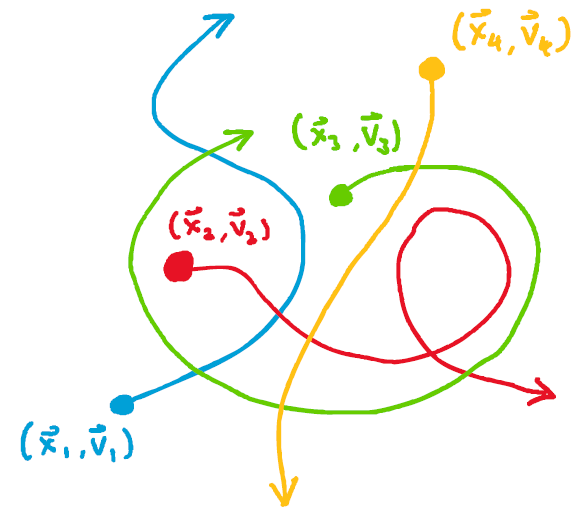
\includegraphics[width=\textwidth]{trajectory}
    \end{minipage}
    \qquad$\Rightarrow$\qquad
    \begin{minipage}{0.2\linewidth}
        \aleq{
            \begin{cases}
                \dv[2]{\vvec{x}_1}{t} = \sum_i F_{i,1}\\[1ex]
                \dv[2]{\vvec{x}_2}{t} = \sum_i F_{i,2}\\
                \phantom{abcde}\vdots\\
                \dv[2]{\vvec{x}_n}{t} = \sum_i F_{i,n}\\
            \end{cases}
        }
    \end{minipage}
\end{center}

The procedure is the same for a system of many-body system. 
E.g. With $1000$ objects, 
their motions can be predicted if we can measure the initial positions and velocities of all $1000$ objects, 
and then solve a system of $1000$ of \nth{2} order differential equations.\\

So the system's state can be uniquely described by $1000$ initial positions and $1000$ initial velocities.
This is an example of \bf{microstate description} - 
the state parameters are properties of individual objects.
\aleq{
    \text{state} = (\vvec{r}_1, \vvec{v}_1, \vvec{r}_2, \vvec{v}_2,..., \vvec{r}_N, \vvec{v}_N)
}

However taking measurement to all objects is impossible in reality. 
As we know that a few ten grams of matter already consist of $\sim 10^{23}$ atoms, 
mechanics picture is not suitable to model large amount of objects.


%%%%%%%%%%%%%%
\subsection{Thermodynamics Picture: Macrostates}

In thermodynamics,
state description is related to overall statistics of the system.
E.g. We have been using the state parameters $(P,V,T)$, which are all statistical quantities:
\begin{itemize}
    \item $P \propto$ \ul{Average} collision force with the container.
    \item $V \propto$ \ul{Average} volume occupied by the gas.
    \item $T \propto$ \ul{Average} velocity of particles. 
\end{itemize}

\begin{center}
    \begin{minipage}{0.4\linewidth}
        \centering
        \includegraphics[height=7em]{AvgV}\\
        If there is no container,\\
        the gas has no fixed volume.
    \end{minipage}
    \hspace{0.05\textwidth}
    \begin{minipage}{0.4\linewidth}
        \centering
        \includegraphics[height=7em]{AvgT}\\
        Maxwell-Boltzmann distribution\\
        at different temperature.
    \end{minipage}
\end{center}

This is the \bf{macrostate description} - 
states are described by the objects' collective behavior instead of looking into them one by one. 
Description by macrostate is much simpler than by microstate because it requires much fewer number of parameters 
(from $\sim 10^{23}$ to less than $10$). 
However this also implies a lost of details about the system.



%%%%%%%%%%%%%%
\subsection{Multiplicity}

Microstates and marcostates are in a many-to-one correspondance:

\begin{itemize}
    \item It we can measure all the microstate parameters, 
    we can calculate the statistical quantities and determine which marcrostate the system is in.

    \item It is impossible to determine the microstate by measuring macrostate parameters, 
    because macrostate description doesn't give fine details. 
    We can have many different configurations (microstates) that yield the same statistical properties (macrostate). 

\end{itemize}

The \bf{multiplicity $W$ of a macrostate} is the number of microstates that correspond to it. 

\begin{center}
    \begin{minipage}{0.7\linewidth}
        \centering
        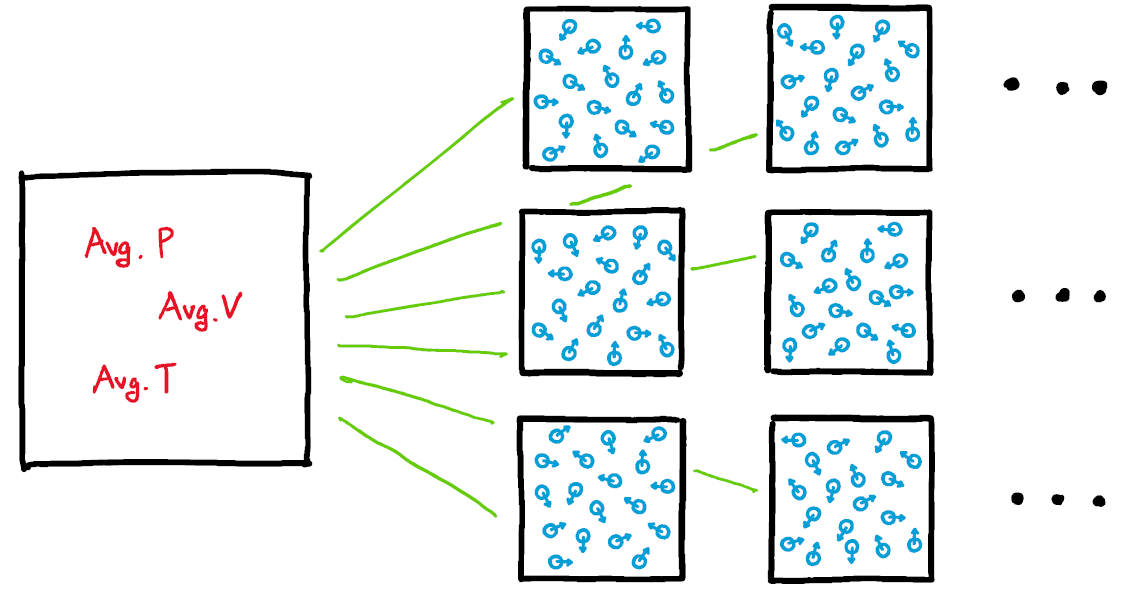
\includegraphics[width=\textwidth]{multiplicity}
    \end{minipage}
\end{center}





\begin{example}
    Suppose we have 4 balls that are allowed to move between 2 boxes $L$ and $R$. What are the 
    \begin{enumerate}
        \item Microstate description?
        \item Macrostate description?
        \item Multiplicity of each macrostate?
    \end{enumerate}

    \begin{center}
        \begin{minipage}{0.95\linewidth}
            \centering
            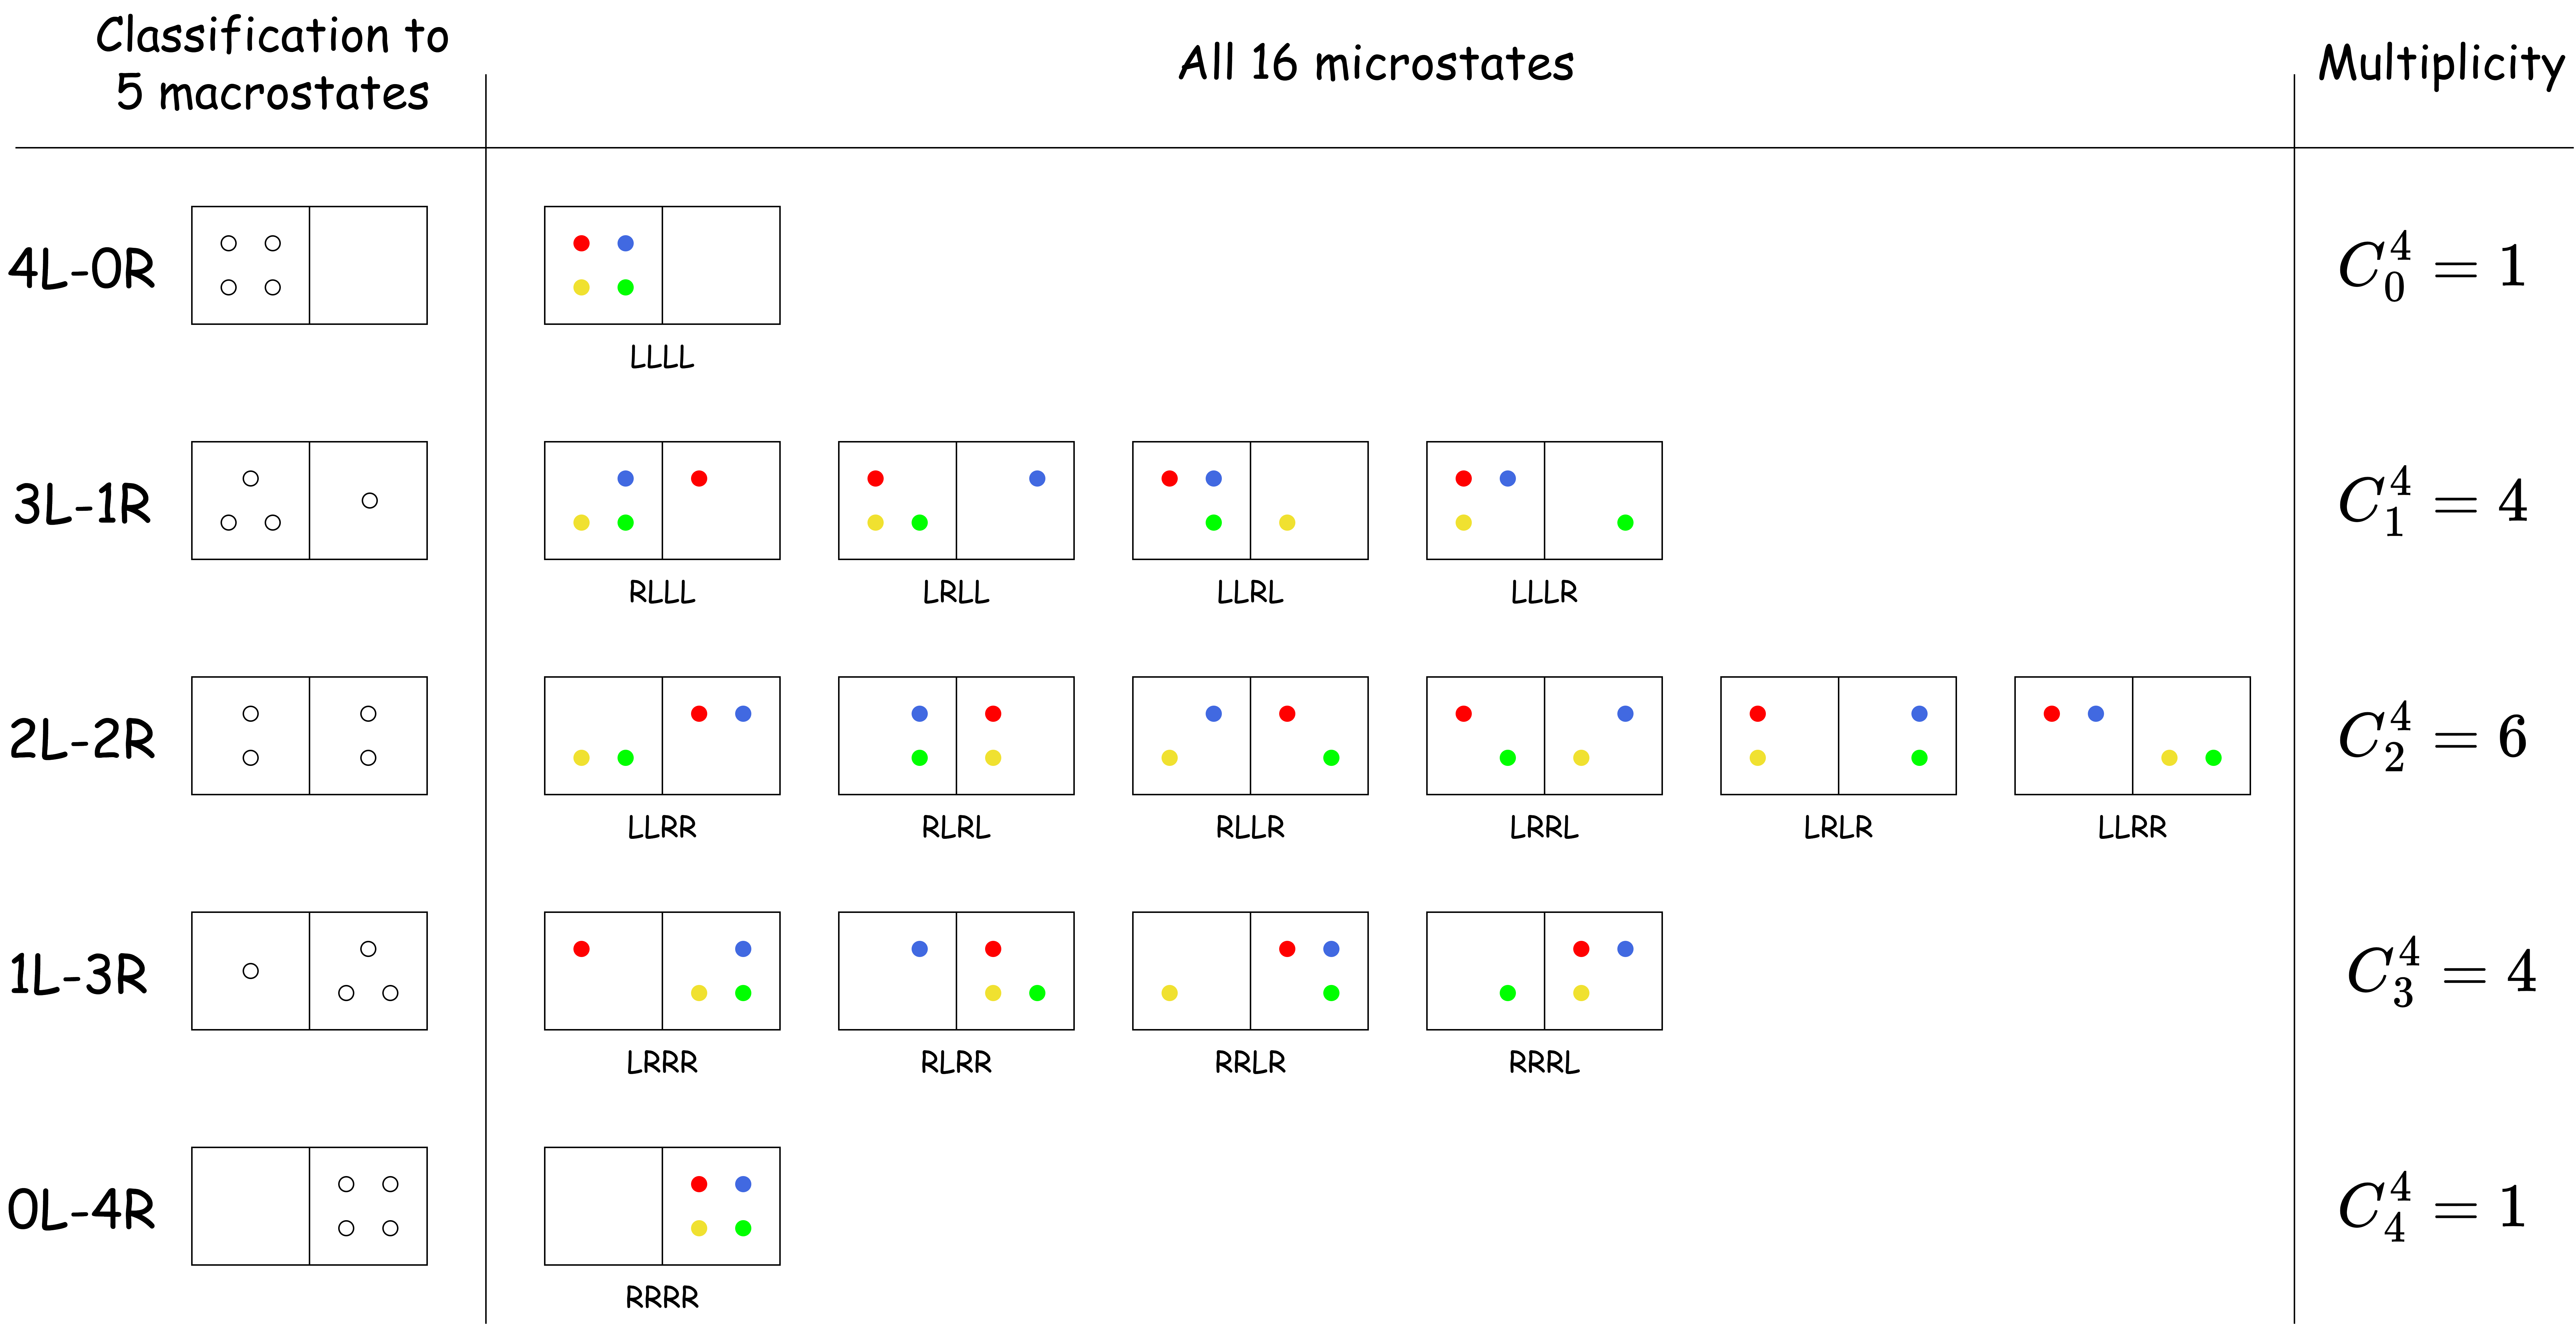
\includegraphics[width=\textwidth]{2box}
        \end{minipage}
    \end{center}

    \begin{enumerate}
        \item For microstate, 
        we have to look at the configuration of the individual balls - 
        for each ball whether it is in the $L$ box or the $R$ box. 
        There are $2^4=16$ different microstates in total.

        \item For macrostate, we look at collective behavior of the balls - 
        how many balls are in the $L$ and $R$ box respectively. 
        There are 5 different kinds of macrostates in total.

        \item By binomial theorem, 
        The multiplicity of each of the macrostates are $C^4_R = \{1,4,6,4,1\}$ respectively,
        where $R$ is the number of balls in the right box. 

    \end{enumerate}
\end{example}



\linesep
% Section %%%%%%%%%%%%%%%%%%%%%%%%%%%%%%%%%%%%%%%%%%%%%%%%%%%%
\section{Boltzmann Entropy}

%%%%%%%%%%%%%%
\subsection{Origin of Irreversibility}

Imagine we allow the balls to move \cul[red]{randomly} between the two boxes. 
\it{Assume} the two boxes to be identical, 
so that each ball should have equal probability to be found in either box. 
Then
\begin{itemize}
    \item Each microstate has an equal probability $\dfrac{1}{16}$ to be found.
    \item The probability of being in a macrostate is proportional to its multiplicity $W$. 
    
\end{itemize}

Therefore, if we take many snapshot from time to time,
we will find that the macrostate 2L-2R has the highest probability $\dfrac{6}{16}$ to be observed.
\begin{center}
    \begin{minipage}{0.4\linewidth}
        \centering
        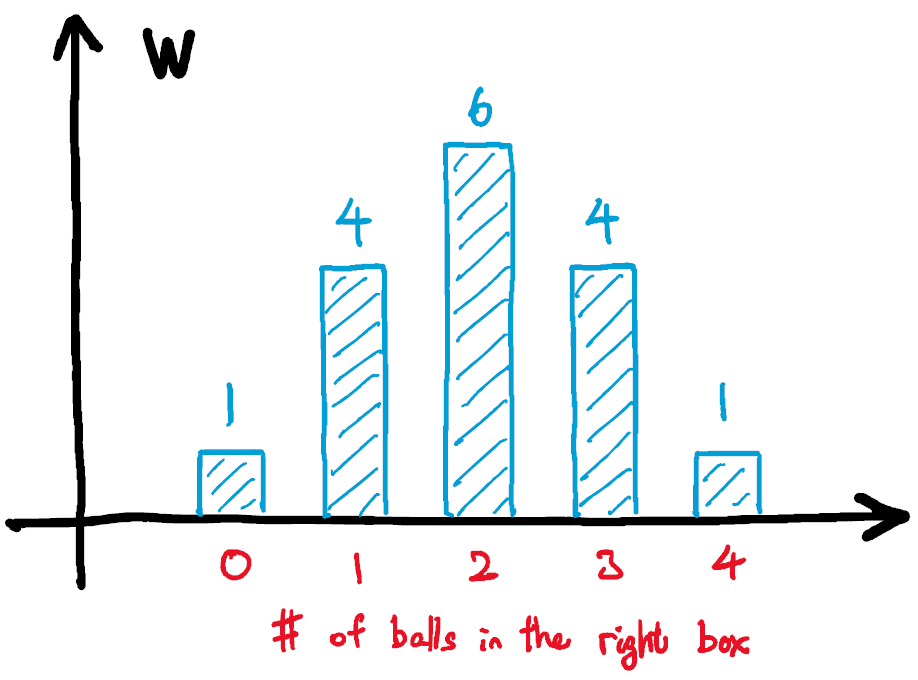
\includegraphics[width=\textwidth]{2box_prob1}
    \end{minipage}
    \quad$\Rightarrow$\quad
    \begin{minipage}{0.4\linewidth}
        \centering
        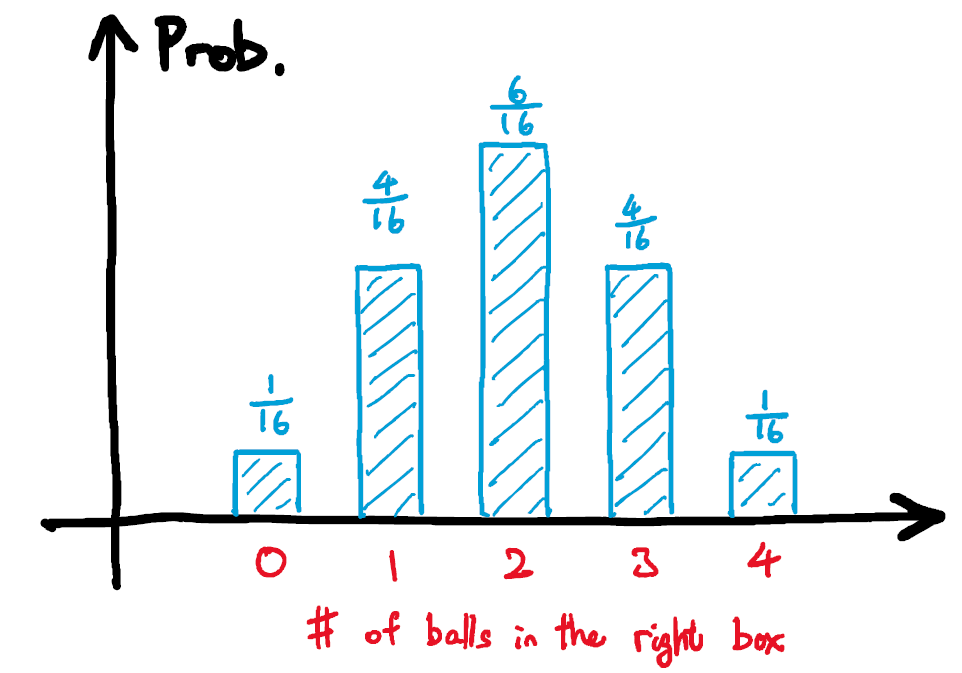
\includegraphics[width=\textwidth]{2box_prob2}
    \end{minipage}
\end{center}

\vskip 1ex
Now consider a more extreme case - 
we begin with $1000$ balls in the $L$ box. 
After allowing the balls to move freely between the boxes,
what will be observed later? 
\begin{itemize}
    \item Multiplicity of macrostate 1000L-0R is $C^{1000}_0 = 1$.
        %so its probability is $\dfrac{1}{2^{1000}} \sim 10^{-301}$.

    \item Multiplicity of macrostate 500L-500R is $C^{1000}_{500} \approx 2.7\times 10^{299}$.
        %so its probability is $\dfrac{C^{1000}_{500}}{2^{1000}} \sim 10^{-2}$.
\end{itemize}

\begin{center}
    \begin{minipage}{0.5\linewidth}
        \centering
        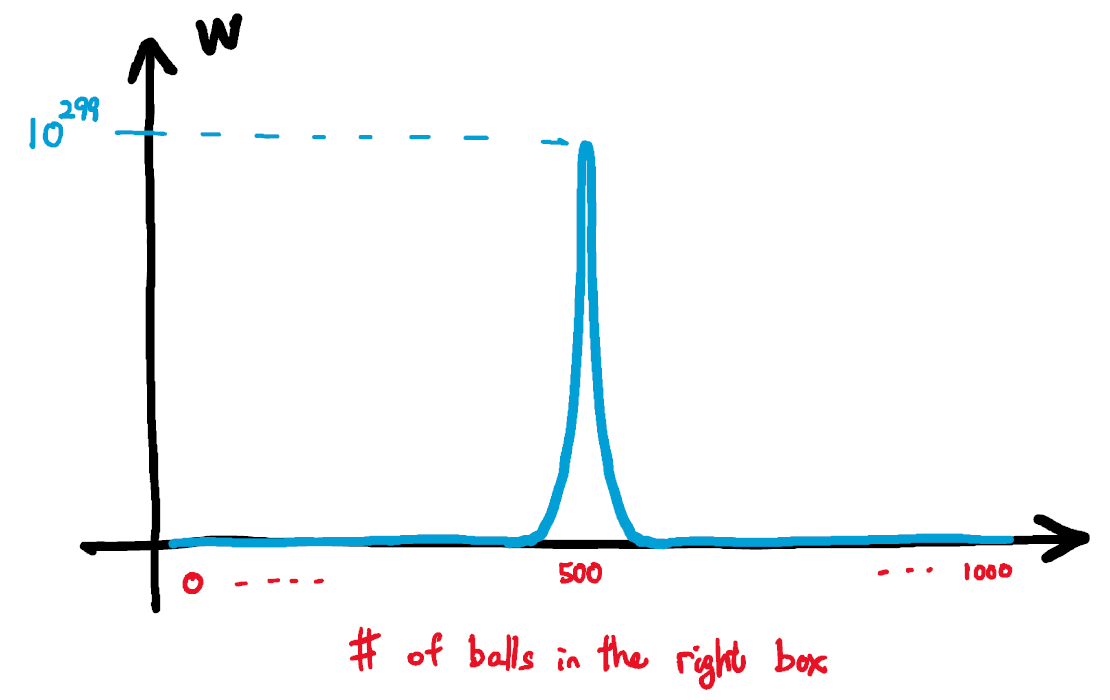
\includegraphics[width=\textwidth]{2box_prob3}
    \end{minipage}
\end{center}

which means on average,
we will observe the balls evenly distributed in two boxes for $\sim 10^{299}$ times before observing them all in one box for 1 time.
Note that the age of our universe is only $\sim 10^{14}$ seconds - 
Even if we are as old as our universe,
1000L-0R state could never be observed.
\begin{itemize}
    \item If it starts at state 1000L-0R, later we will observe it evolves into state 500L-500R.
    \item If it starts at state 500L-500R, we will (almost) never see it evolves into state 1000L-0R.
\end{itemize}

\begin{center}
    \red{This is the truth of irreversibility!}
\end{center}

Technically all processes are reversible,
but it takes a \it{really long} time for the reverse to happen.

\vskip 1em
%%%%%%%%%%%%%%
\subsection{Boltzmann's Hypothesis}

Summarizing what we have learnt:
\begin{itemize}
    \item Clausius found a function $S$, 
    which the change $\Delta S \geq 0$ in every closed system (energy conserved within).

    \item According to probability, 
    system always evolves from marcostate with low multiplicity to macrostate with high multiplicity.
    The reverse (almost) never happens.
\end{itemize}

So a smart guy, 
\href{https://en.wikipedia.org/wiki/Ludwig_Boltzmann}{Ludwig Boltzmann} proposed the relation:
\aleq{
    \tkn{boltz_S}{\cul[red]{S}} = \tkn{boltz_phi}{\cul[blue]{\phi}}(\tkn{boltz_W}{\cul[green]{W}})
}
\addArrow[red]{boltz_S}{(-5ex,-3ex)}{\scriptsize Entropy}{(0,-1ex)}
\addArrow[blue]{boltz_phi}{(0,-3ex)}{\scriptsize Some relation\\[-1ex]\scriptsize to be determined}{(0,-1.5ex)}{(0,-1ex)}
\addArrow[green]{boltz_W}{(7ex,-3ex)}{\scriptsize Multiplicity}{(0,-1ex)}{(1ex,0)}

\vskip 2em
What mathematical requirements should $\phi(\cdot)$ satisfy?
Consider combining two 2-boxes systems $A$ and $B$,
each with different colour of balls.
Their individual macrostate are denoted with multiplicity $W_A$ and $W_B$ respectively.

\begin{center}
    \begin{minipage}{0.3\linewidth}
        \centering
        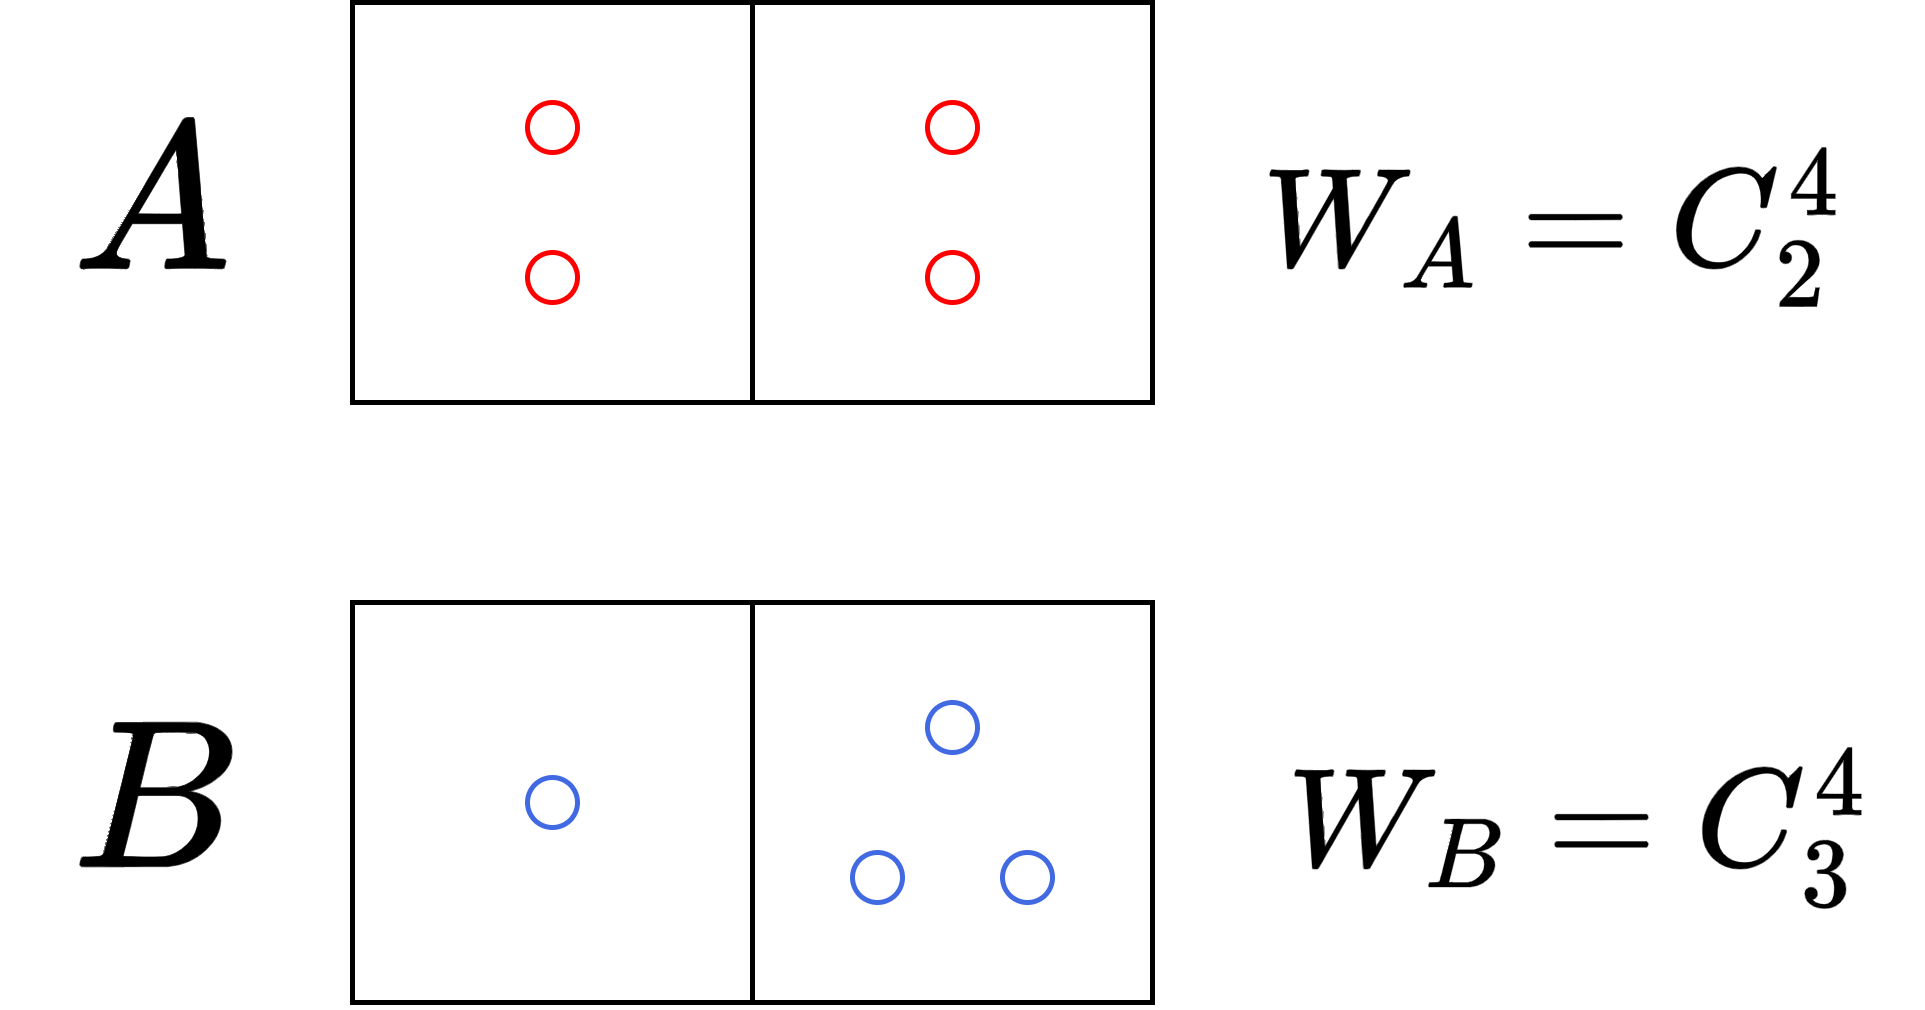
\includegraphics[width=\textwidth]{2box_combine1}
    \end{minipage}
    \qquad$\Rightarrow$\qquad
    \begin{minipage}{0.45\linewidth}
        \centering
        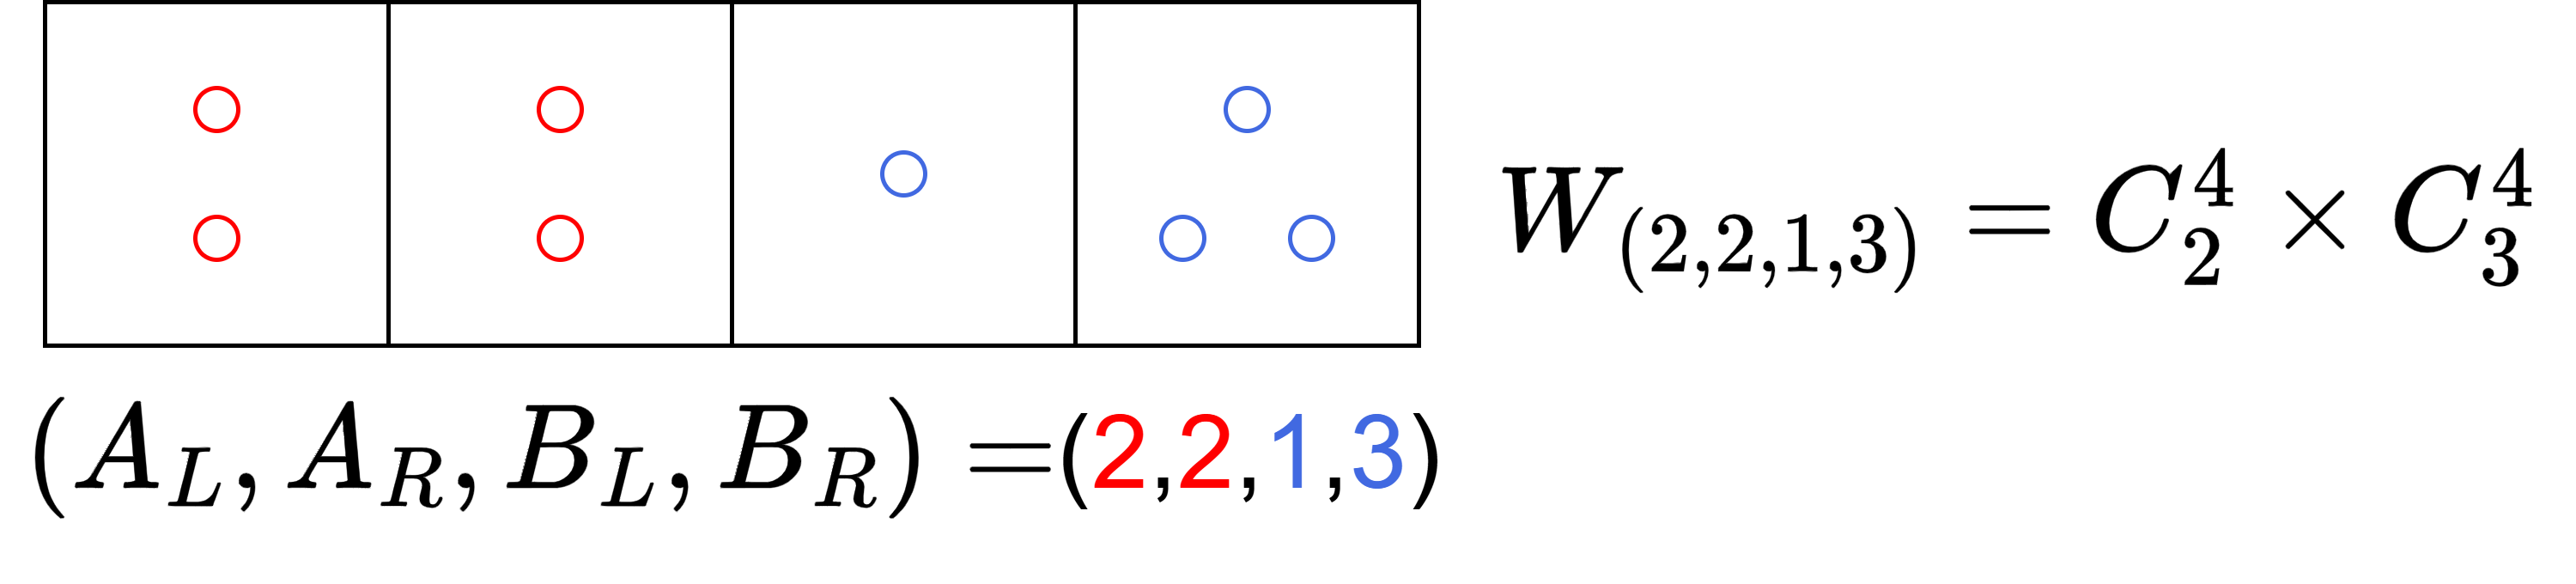
\includegraphics[width=\textwidth]{2box_combine2}
    \end{minipage}
\end{center}

\begin{itemize}
    \item Recall that total $S$ of multiple objects is calculated by addition.
    \aleq{
        S_\text{total} = S_A + S_B = \phi(W_A) + \phi(W_B)
    }

    \item If we look at them as a combined system,
    because calculating multiplicity is just counting the number of combination,
    \aleq{
        W_\text{total} &= \qty(\mstack{\text{\# of ways}\\\text{to arrange balls}\\\text{in box A}})
        \times \qty(\mstack{\text{\# of ways}\\\text{to arrange balls}\\\text{in box B}})\\[1ex]
        &= W_A \times W_B\\[1ex]
        \Rightarrow\quad S_\text{total} &= \phi(W_A\times W_B)
    }
\end{itemize}

What function(s) satisfy such relation $\phi(W_A)+\phi(W_B) = \phi(W_A\times W_B)$?
\bf{Logarithm}.
\aleq{
    \ln(W_A) + \ln(W_B) = \ln(W_A\times W_B)
}

This is how we arrive at the Boltzmann's entropy hypothesis:
\aleq{
    \Aboxed{
        S = \tkn{boltz_k}{\cul[red]{k}}\ln W
    }
}
\addArrow[red]{boltz_k}{(0,-3ex)}
{$k =$ Some proportionality constant we don't know yet}
{(0,-0.5ex)}


%%%%%%%%%%%%%%
\subsection{Finding Boltzmann Constant}

Now it comes to the question of what value should we take for $k$. 
Ideal gas, the system being most familiar by physicists, 
is used to set the baseline. 

\begin{enumerate}
    \item Firstly, consider the gas expanding under an isothermal process.
    The entropy change is
    \aleq{
        \Delta S = \int \frac{\var{Q}}{T} = nR\ln\qty(\frac{V_2}{V_1})
    }

    \item Change in multiplicity on an isotheral path can be modelled by
    \begin{enumerate}
        \item[2.1.] Divide the box volume $V_1$ into unit cells of (arbituary) volume $\Delta V$.
        \begin{center}
            \begin{minipage}{0.4\linewidth}
                \centering
                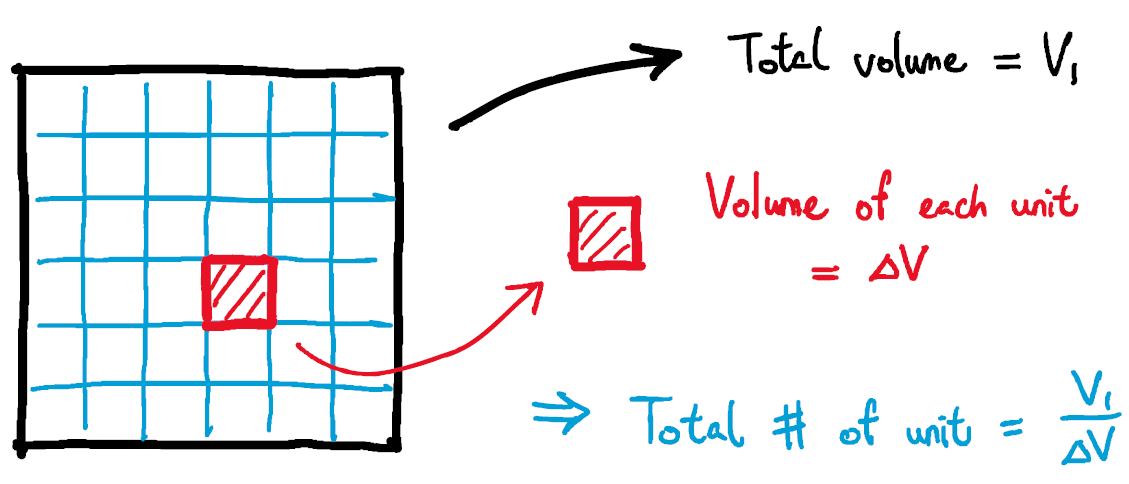
\includegraphics[width=\textwidth]{gas_partition1}
            \end{minipage}
        \end{center}

        \item[2.2.] Put $n$ particles in the box. Then
        \begin{itemize}
            \item \# of ways to put 1 particle $=\dfrac{V_1}{\Delta V}$
            \item \# of ways to put $N$ particles $=\qty(\dfrac{V_1}{\Delta V})^N$
        \end{itemize}
        So the multiplicity is proportional to $W_1 \propto \qty(\dfrac{V_1}{\Delta V})^N$.

        \item[2.3.] Let the box expand to volume $V_2$. 
        Now there are more unit cells in the box.
        \begin{center}
            \begin{minipage}{0.5\linewidth}
                \centering
                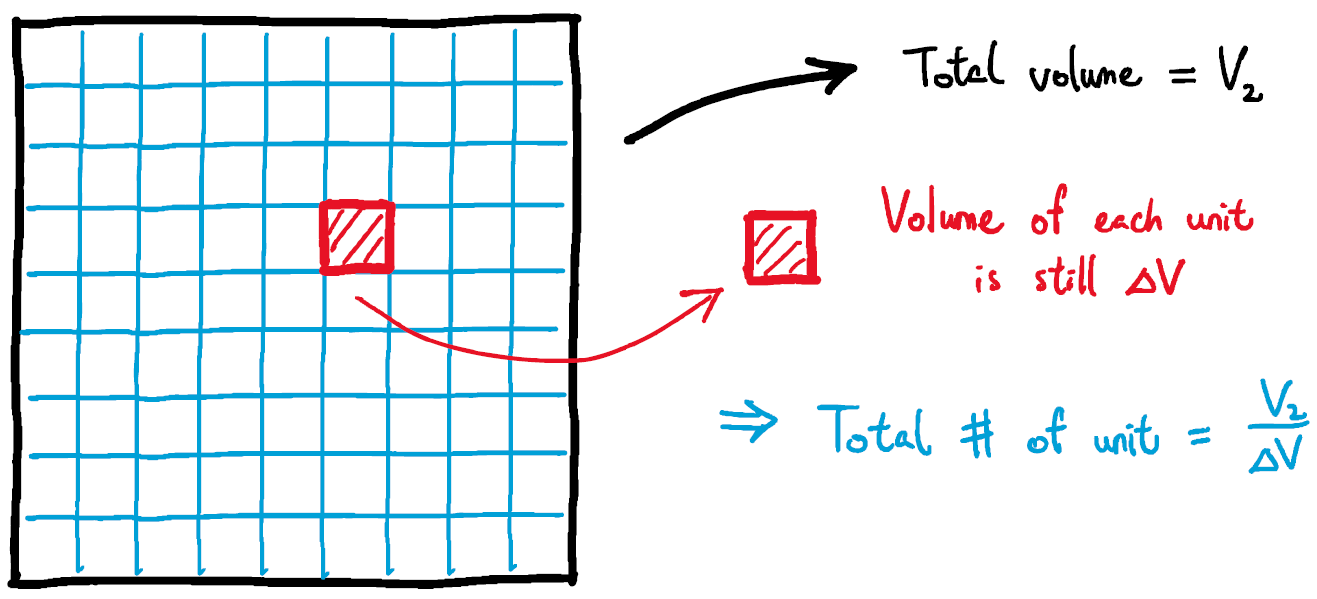
\includegraphics[width=\textwidth]{gas_partition2}
            \end{minipage}
        \end{center}
        \begin{itemize}
            \item \# of ways to put 1 particle $=\dfrac{V_2}{\Delta V}$
            \item \# of ways to put $N$ particles $=\qty(\dfrac{V_2}{\Delta V})^N$
        \end{itemize}
        So the multiplicity increases to $W_2 \propto \qty(\dfrac{V_2}{\Delta V})^N$.
    \end{enumerate}

    \item Plugging in the above into the formula $S=\ln(W)$,
    \addArrow[red]{S_n}{(-5ex,-2ex)}
    {\scriptsize \# of particle\\[-1ex]\scriptsize but in moles}{(-1ex,-1ex)}{(-3ex,-1ex)}
    \addArrow[green]{S_R}{(0,-2ex)}{\scriptsize Ideal gas\\[-1ex]\scriptsize constant}{(0,-1ex)}{(0,-1ex)}
    \addArrow[blue]{S_N}{(5ex,-2ex)}{\scriptsize \# of particle}{(1ex,-1ex)}{(4ex,0)}
    \addBentArrow[yellow]{S_NA}{(7ex,-2ex)}{\scriptsize Avogadro's number}{(0,-1.5ex)}{(5.5ex,1ex)}
    \aleq{
        \Delta S &= S_2 - S_1\\
        nR\ln\qty(\frac{V_2}{V_1}) &= k\ln(W_2) - k\ln(W_1) \\
        &= k\ln\qty[\frac{\frac{V_2}{\Delta V}}{\frac{V_1}{\Delta V}}]\\
        &= Nk\ln\qty(\frac{V_2}{V_1})\\
        \tkn{S_n}{\cul[red]{n}}\tkn{S_R}{\cul[green]{R}} &= \tkn{S_N}{\cul[blue]{N}}k\\[3em]
        k &= \frac{R}{\tkn{S_NA}{\cul[yellow]{N_A}}}
        \approx 1.38\times 10^{-23}
    }
\end{enumerate}

\newpage
\begin{example}
    We can use Boltzmann's entropy formula to estimate the change multiplicity in real life process,
    to see how much "irreversible" they are.
    \aleq{
        \Delta S = k\ln(\Delta W)
        \qquad \Rightarrow \qquad 
        \Delta W = e^{\frac{\Delta S}{k}}
    }

    Suppose we have 2 objects with the same heat capacity $C=1$,
    but object A is at $300.1$ K and object B is at $299.9$ K.
    After allowing heat exchange,
    we expect both reaching the equilibrium temperature $300$ K.
    The entropy change in this process is 
    \aleq{
        &\bcase{
            \Delta S_A &= \int^{300}_{300.1} \frac{C\dd{T}}{T} = C\cdot \ln\qty(\frac{300}{300.1})\\
            \Delta S_B &= \int^{300}_{299.9} \frac{C\dd{T}}{T} = C\cdot \ln\qty(\frac{300}{299.9})\\
        }\\[1em]
        %
        \Rightarrow\quad &\Delta S_\text{total} = C\cdot \ln\qty(\frac{300}{300.1}\cdot \frac{300}{299.9}) \approx 1.11\times 10^{-7}\\[1ex]
        %
        &\Delta W = \frac{W_\text{final}}{W_\text{initial}} = e^{\frac{\Delta S}{k}} = e^{8.05\times 10^{15}} \approx 10^{10^{15.54}}
    }

    The multiplicity has increased by a ratio of a number with $10^{15}$ digits.
    This is physically equivenlently to say that the reverse process will never be observed.
\end{example}

%%%%%%%%%%%%%%
\subsection{Entropy as Disorderness}

In physics books, 
we usually regards entropy as disorderness due to Boltzmann hypothesis - 
because there are more ways to make things look messy than to make things look tidy.
\begin{itemize}
    \item A tidy place = Everything is in its fixed position. 
    E.g. Clothes should be in wardrobes and books should be on bookshelves.
    Multiplicity is low, and so entropy is low.

    \item A messy place = Many randomness. 
    E.g. You can put your clothes anywhere other than wardrobes if you want your room looks messy.
    Multiplicity is high, and so entropy is high.
\end{itemize}

\begin{center}
    \begin{minipage}{0.4\linewidth}
        \centering
        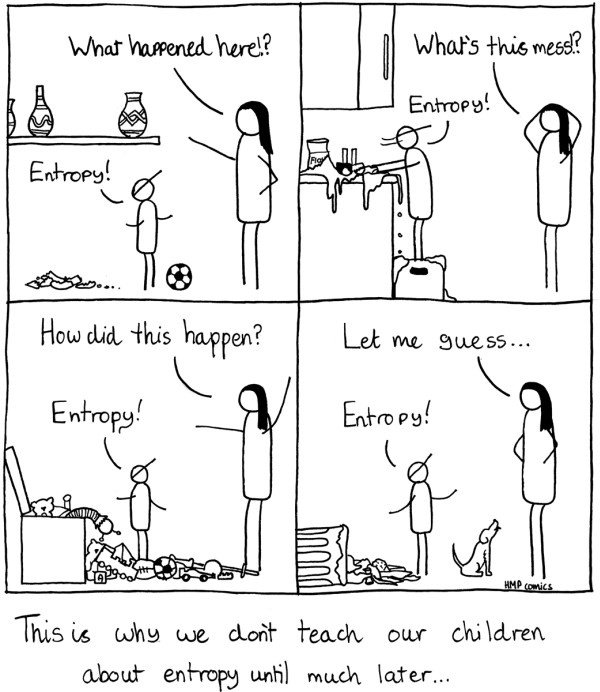
\includegraphics[width=\textwidth]{comic}
    \end{minipage}
\end{center}


\linesep
% Section %%%%%%%%%%%%%%%%%%%%%%%%%%%%%%%%%%%%%%%%%%%%%%%%%%%%
\section{A Temperature Scale by Entropy}

Let's recap some temperature scales we know in history:
\begin{enumerate}
    \item \ul{Emperical scales}: A linear interpolation between two fixed reference point. E.g.
    \begin{itemize}
        \item \href{https://en.wikipedia.org/wiki/Anders_Celsius}{Celsius} (1701-1744) : 
        Between water's freezing point ($0^\circ$C) and boiling point ($100^\circ$C)

        \item \href{https://en.wikipedia.org/wiki/Daniel_Gabriel_Fahrenheit}{Fahrenheit} (1686-1736) :
        Between the eutectic temperature of ammonium chloride brine ($0^\circ$F) and average human body temperature ($96^\circ$F)
        
    \end{itemize}

    Thermometers in these scales measure temperature using material expansion under heat,
    which limit the scale by the freezing point of the measuring material.

    \item \ul{Thermodynamics scale}: A theoretical scale based entirely based on macroscopic properties of material.
    i.e. Kelvin scale based on relation with Carnot engine's efficiency.

    \begin{itemize}
        \item The first scale that defines the full temperature range $-273.15^\circ$C to $\infty^\circ$C.
        \item Prove that going below $-273.15^\circ$C is not physical.
    \end{itemize}
    
\end{enumerate}

However after entropy is established as a state function,
physicists find a new mathematical way to define temperature - 
through the relation between internal energy and entropy.
\begin{itemize}
    \item We previously write internal energy $U$ of a material as a state function of 3 variables $(P,V,T)$,
    but only two of them are independent because there is the equation of state (e.g. ideal gas law).

    \item Entropy is also a function of $(P,V,T)$.
\end{itemize}

It should not make a different if we do a change of variable,
making internal energy as a function of 4 variables $(P,V,T,S)$!
\aleq{
    U = U(P,V,T,S) 
    \qquad\text{with}\qquad 
    \text{only }2\text{ of the variables independent}
}

Let's say if we choose the two independent ones to be $V$ and $S$,
\begin{itemize}
    \item According to the thermal \nth{1} law,
    \aleq{
        \dd{U} = \var{Q} - \var{W} = T\dd{S} - P\dd{V}
    }

    \item By partial differentiation chain rule,
    \aleq{
        \dd{U(S,V)} = \qty(\pdvv{U}{S})\dd{S} + \qty(\pdvv{U}{V})\dd{V}
    }
\end{itemize}

$T$ and $P$ appears as functions of $(S,V)$,
giving us new way of defining them.
\aleq{
    T(S,V) \ \defeq\  \pdvv{U}{S}
    \quad,\quad
    P(S,V) \ \defeq\  -\pdvv{U}{V}
}

\begin{center}
    \red{If we can measure a material's internal energy and entropy,
    plot them on a graph,\\ 
    then temperature of the material can be defined using the slope of the $U$-$S$ graph.}
\end{center}

However, because $U$ is usaually some simple function and easy to compute,
while $S$ needs to be computed by multiplicity (i.e. a lot of combinatorics),
it is easier to define $T$ by differentiating in the reverse way:
\aleq{
    \Aboxed{
        \inv{T} \ \defeq\ \pdvv{S}{U}
    }
}


\begin{notation}
    In some advanced thermodynamics textbooks, 
    the definition may be subscripted in the following way:
    \aleq{
        T(S,V) \ \defeq\  \qty(\pdvv{U}{S})_\text{\blue{const. V}}
        \quad,\quad
        P(S,V) \ \defeq\  -\qty(\pdvv{U}{V})_\text{\blue{const. S}}
    }

    This is just for emphasizing which of the $(P,V,T,S)$ is the another independent variable,
    which must be kept constant in the partial differentiation.

\end{notation}

\vskip 1em
By this temperatue - internal energy - entropy relation,
we can derive some interesting properties about non-ideal gas materials.
\begin{enumerate}
    \item Count multiplicity by some state parameter $x$. 
    $x$ is specific to the material.
    Then compute $S = k\ln W$

    \item Express $U$ as a function of $x$.
    
    \item A relation is born by relate $S$ and $U$ by $T$.
    \aleq{
        \inv{T} = \pdvv{S}{U} 
        = \dfrac{\qty(\pdvv{S}{x})}{\qty(\pdvv{U}{x})}
    }

\end{enumerate}

\vskip 1em
%%%%%%%%%%%%%%
\subsection{Example 1: Crystal Vaccancy Model}

A crystal is a regular arrangement of atoms/molecules.\\

\ul{Perfect crystal} : There is only 1 possible arrangement.
        $\Rightarrow$ Multiplicity $=1$
\begin{center}
    \begin{minipage}{0.3\linewidth}
        \centering
        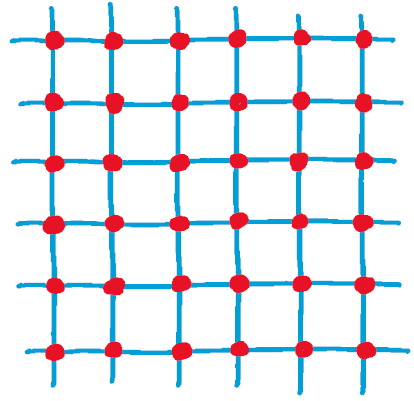
\includegraphics[width=0.75\textwidth]{crystal_perfect}
    \end{minipage}
\end{center}

\newpage
\ul{Crystal with defect} : There are many possibilities to introduce defects.
$\Rightarrow$ High multiplicity
\begin{center}
    \begin{minipage}{0.3\linewidth}
        \centering
        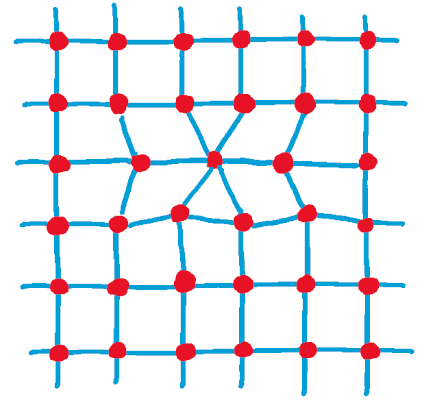
\includegraphics[width=0.75\textwidth]{crystal_missing}\\
        Vaccancy (missing atoms)
    \end{minipage}
    \hspace{0.05\textwidth}
    \begin{minipage}{0.3\linewidth}
        \centering
        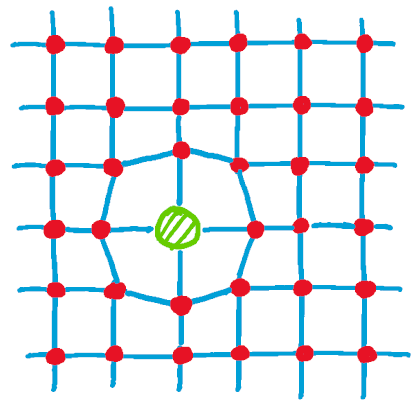
\includegraphics[width=0.75\textwidth]{crystal_impure}\\
        Substitution by impurities
    \end{minipage}
\end{center}

\vskip 1ex
In a crystal with defect, 
we also expect there is a energy change per defect because 
the atomic bondings around the defect are different.
Thus we can use the $T$-$S$-$U$ relation
to model the expected number of defects.

\begin{enumerate}
    \item Suppose we have a crystal with a total $N+n$ sites,
    $N$ being the crystal's atoms and $n$ being substitute by impurity/vaccancy.
    Then the multiplicity is the number of ways to arrange $N$ atoms into $N+n$ positions.
    \aleq{
        W = C^{N+n}_n = \frac{(N+n)!}{N!n!}
    }

    \item Calculating the Boltzmann entropy:
    \aleq{
        S &= k\ln\qty(\frac{(N+n)!}{N!n!}) \\
        &= k\qty[\ln (N+n)! - \ln N! - \ln n!] \\
        &\approx k\qty[(N+n)\ln(N+n) - N\ln N - n\ln n]
    }
    Here we have used the \bf{Stirling approximation}:
    \fbox{$\ln N! \approx N\ln N - N$}, 
    which applies when $N$ is a very big number.

    \item \it{Assume} that each impurity/vaccancy brings an increase of internal energy by $\epsilon$,
    which $\epsilon$ may be some values measurable from experiments.
    A total $n$ sites of impurity/vaccancy gives a total internal energy 
    \aleq{
        U = n\epsilon
    }

    \item Finally, apply the $T$-$S$-$U$ relation.
    We observe that both $S$ and $U$ are functions of $n$,
    \aleq{
        \pdvv{S}{n} &= k\pdvv{n}\qty[(N+n)\ln (N+n) - N\ln N - n\ln n]\\
        &= k\qty[\ln (N+n) - \ln n]\\
        &= k \ln \qty(\frac{N+n}{n})\\[1ex]
        %
        \pdvv{U}{n} &= \pdvv{n}n\epsilon = \epsilon\\[1ex]
        %
        \Rightarrow\quad \inv{T} = \pdvv{S}{U} 
        &= \dfrac{\qty(\pdvv{S}{n})}{\qty(\pdvv{U}{n})}
        = \frac{k}{\epsilon}\ln \qty(\frac{N+n}{n})
    }
\end{enumerate}

By a change of subject, we get
\aleq{
    (\text{Portion of defects}) = \frac{n}{N} = 
    \dinv{e^{-\frac{\epsilon}{kT}} - 1}
}
Observe that $n\to 0$ only if $T\to 0$,
meaning that crystal in real life must have some defects (statistically).
\cul[red]{Crystal can spontaneously form defects under normal temperature}.


%%%%%%%%%%%%%%
\subsection{Example 2: Rubber Band Contraction}

A rubber band can be considered a long chain of atom (e.g. polymer).\\

\ul{Full extension} : The string is completely straight.
There is only 1 possible arrangement. 
$\Rightarrow$ Multiplicity $=1$.

\begin{center}
    \begin{minipage}{0.55\linewidth}
        \centering
        
\includegraphics[width=\textwidth]{rubber_straight}
    \end{minipage}
\end{center}


\ul{Entangled state} : The string curled up and the total length shorten.
Have many possible arrangements.
$\Rightarrow$ High multiplicity.

\begin{center}
    \begin{minipage}{0.4\linewidth}
        \centering
        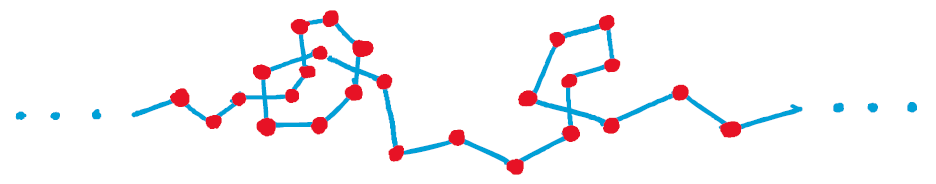
\includegraphics[width=\textwidth]{rubber_curl}
    \end{minipage}
\end{center}

For simplicity, we only consider a 1D chain - 
the connections to next atom can only be pointing left or right.

\begin{center}
    \begin{minipage}{0.6\linewidth}
        \centering
        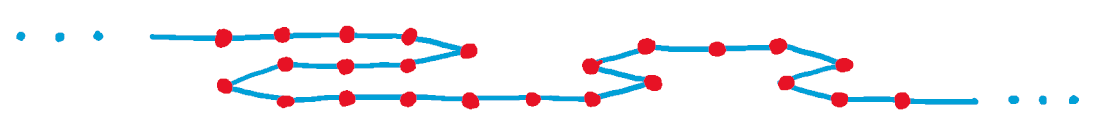
\includegraphics[width=\textwidth]{rubber_1D}
    \end{minipage}
\end{center}

\begin{enumerate}
    \item Suppose the chain has $N+1$ atoms (so a total of $N$ connections).
    There are $n_L$ connections pointing to the left and 
    $N-n_L$ connections pointing to the right.
    Then the multiplicity is the number of ways to assign $n_L$ left connections out of the total $N$ connections.
    \aleq{
        W = C^N_{n_L} = \frac{N!}{n_L!(N-n_L)!}
    }

    \begin{center}
        \begin{minipage}{0.6\linewidth}
            \centering
            
\includegraphics[width=\textwidth]{rubber_1D_arrow}
        \end{minipage}
        \hspace{0.05\textwidth}
        \begin{minipage}{0.2\linewidth}
            \centering
            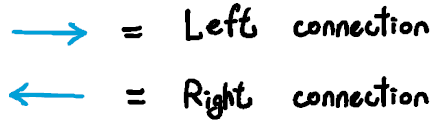
\includegraphics[width=\textwidth]{rubber_1D_connect}
        \end{minipage}
    \end{center}

    \item Calculating the Boltzmann entropy:
    \aleq{
        S &= k\ln\qty(\frac{N!}{n_L!(N-n_L)!}) \\
        &= k\qty[\ln N! - \ln n_L! - \ln (N-n_L)!] \\
        &\approx k\qty[N\ln N - n_L\ln n_L - (N-n_L)\ln (N-n_L)]
    }
    Again, the Stirling approximation formula is used here.

    \item We can relate the internal energy in a rubber band with its stored elastic energy.
    Let the connection between atoms be of length $d$, 
    such that the total length of the chain is $[n_L - (N-n_L)]\times d = (2n_L-N)d$.
    When a tension $F$ is applied on both side of the chain
    to unfold 1 right connection into 1 left connection,

    \begin{center}
        \begin{minipage}{0.3\linewidth}
            \centering
            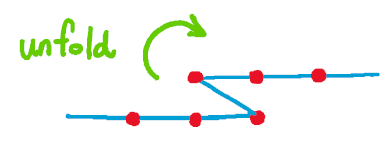
\includegraphics[width=\textwidth]{rubber_unfold1}
        \end{minipage}
        \qquad$\Rightarrow$\qquad
        \begin{minipage}{0.4\linewidth}
            \centering
            
\includegraphics[width=\textwidth]{rubber_unfold2}
        \end{minipage}
    \end{center}

    \begin{itemize}
        \item Number of left connection $n_L \rightarrow n_L+1$.
        \item Total length of the chain $(2n_L-N)d \rightarrow (2n_L-N)d+2d$.
        \item The work done by the tension is $F\cdot 2d$
    \end{itemize}

    Denote $\Delta n$ as the number of right connection being unfolded into left connection,
    then 
    \aleq{
        \pdvv{n_L}{(\Delta n)} &\approx \frac{(n_L+\Delta n)-n_L}{\Delta n} = 1\\[1ex]
        \pdvv{U}{(\Delta n)} = \pdvv{(W.D.)}{(\Delta n)} &\approx \frac{(F+2Fd(\Delta n))-F}{\Delta n} = 2Fd 
    }

    \vskip 1ex
    \item Finally, apply the $T$-$S$-$U$ relation.
    We observe that both $S$ and $U$ are functions of $\Delta n$
    \aleq{
        \pdvv{S}{(\Delta n)} &= \dvv{S}{n_L}\pdvv{n_L}{(\Delta n)}\\
        &= k \qty[\ln(N-n_L) - \ln n_L] \cdot 1\\
        &= k\ln \qty(\frac{N-n_L}{n_L})\\[1ex]
        %
        \pdvv{U}{(\Delta n)} &= 2Fd \\[1ex]
        %
        \Rightarrow\quad \inv{T} = \pdvv{S}{U} 
        &= \dfrac{\qty(\pdvv{S}{n})}{\qty(\pdvv{U}{n})}
        = \frac{k}{2Fd}\ln \qty(\frac{N-n_L}{n_L})
    }

\end{enumerate}

Substitute by the length of the chain $L=(2n_L-N)d$ and change of subject to $F$, we get
\aleq{
    (\text{Tension}) = F = 
    \frac{kT}{2d}\ln\qty(\frac{Nd+L}{Nd-L})
}
Observe that when $L$ is kept constant,
$F$ increases if $T$ increases.
\cul[red]{The rubber band would} \cul[red]{like to contract under heat!}

\newpage
%%%%%%%%%%%%%%
\subsection{Negative Temperature?}

In our new definition of temperature
\aleq{
    \dinv{T} = \pdvv{S}{U} 
    = \qty(\mstack{\text{Rate of change of entropy}\\\text{with respect to energy}})
}

if there is a system whose entropy decreases ($S\downarrow$) 
when its internal energy increases ($U\uparrow$), 
$\dinv{T} = \pdvv{S}{U}<0$, i.e. negative temperature.

\begin{center}
    \red{Negative temperature happens only in systems with finite number of microstate.}
\end{center}

For example, let's revisite the 2 boxes system.
But this time we assign potential energy difference between the boxes -
balls in the right box would have higher energy than in the left box by $\epsilon$.

\begin{center}
    \begin{minipage}{0.35\linewidth}
        \centering
        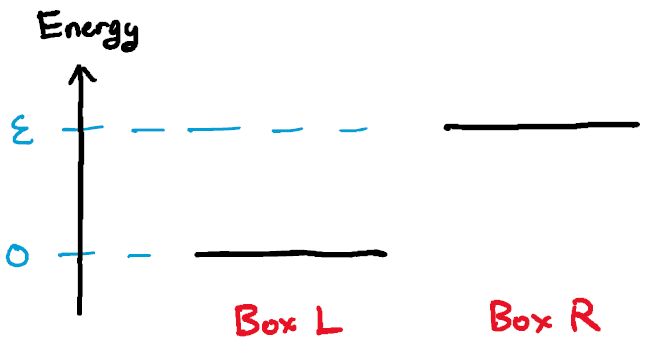
\includegraphics[width=\textwidth]{2box_E0}
    \end{minipage}
\end{center}

\begin{minipage}{0.6\linewidth}
    \begin{itemize}
        \item When total energy $=3\epsilon$,
        there are 4 possible \\ microstates.
        Entropy $\sim \ln(4) = 1.38$.
    \end{itemize}
\end{minipage}
\hspace{0.03\textwidth}
\begin{minipage}{0.35\linewidth}
    \centering
    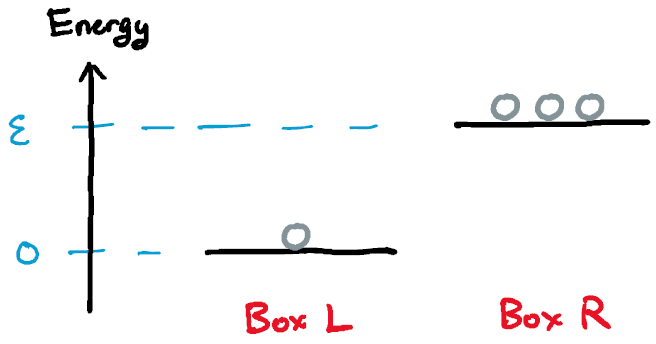
\includegraphics[width=\textwidth]{2box_E4}
\end{minipage}

\begin{minipage}{0.6\linewidth}
    \begin{itemize}
        \item When total energy increases to $4\epsilon$,
        there is only 1 possible microstates.
        Entropy decreases to $\sim \ln(1) = 0$.
    \end{itemize}
\end{minipage}
\hspace{0.03\textwidth}
\begin{minipage}{0.35\linewidth}
    \centering
    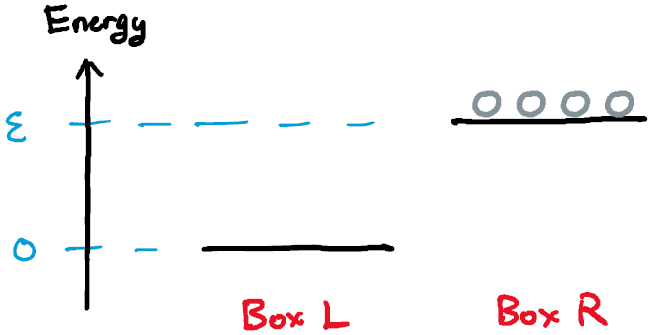
\includegraphics[width=\textwidth]{2box_E5}
\end{minipage}

\vskip 1em
Plotting the graph of $W$ and $S$ against internal energy $U$ respectively: 
\begin{center}
    \begin{minipage}{0.4\linewidth}
        \centering
        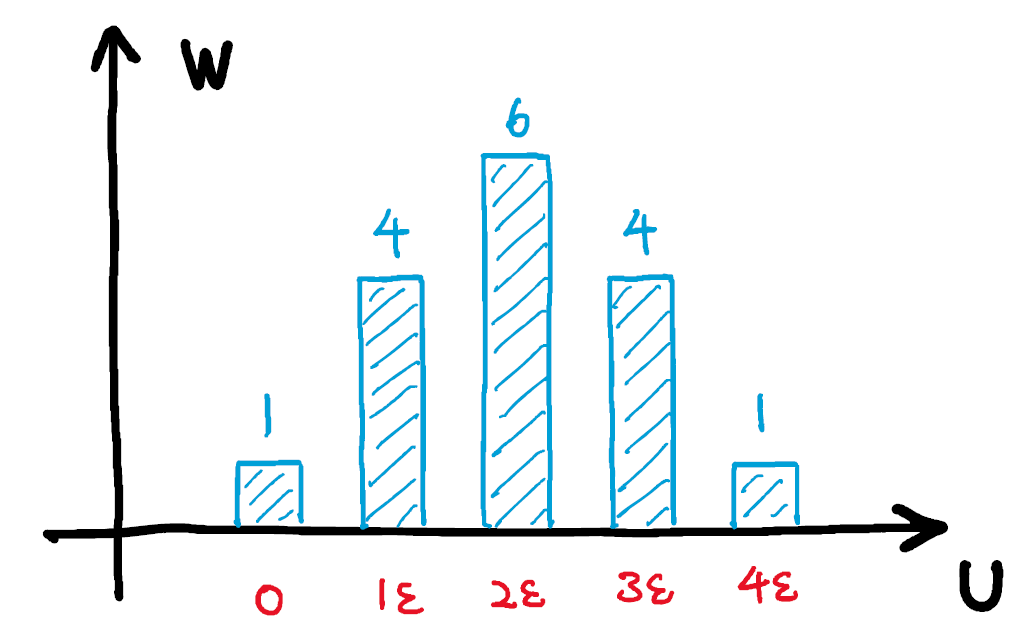
\includegraphics[width=\textwidth]{WU1}
    \end{minipage}
    \quad{\huge $\Rightarrow$}\quad
    \begin{minipage}{0.4\linewidth}
        \centering
        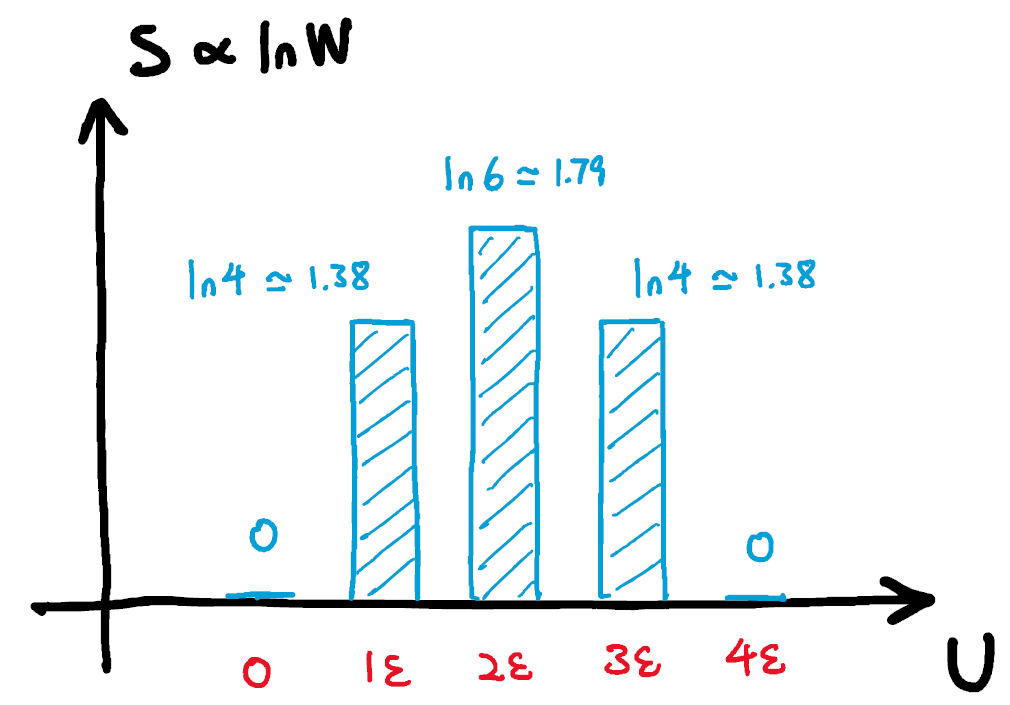
\includegraphics[width=\textwidth]{WU2}
    \end{minipage}
\end{center}

\newpage
In cases where the internal energy can be taken as continuous values,
the $S$-$U$ graph will become a smooth curve like so:

\begin{center}
    \begin{minipage}{0.8\linewidth}
        \centering
        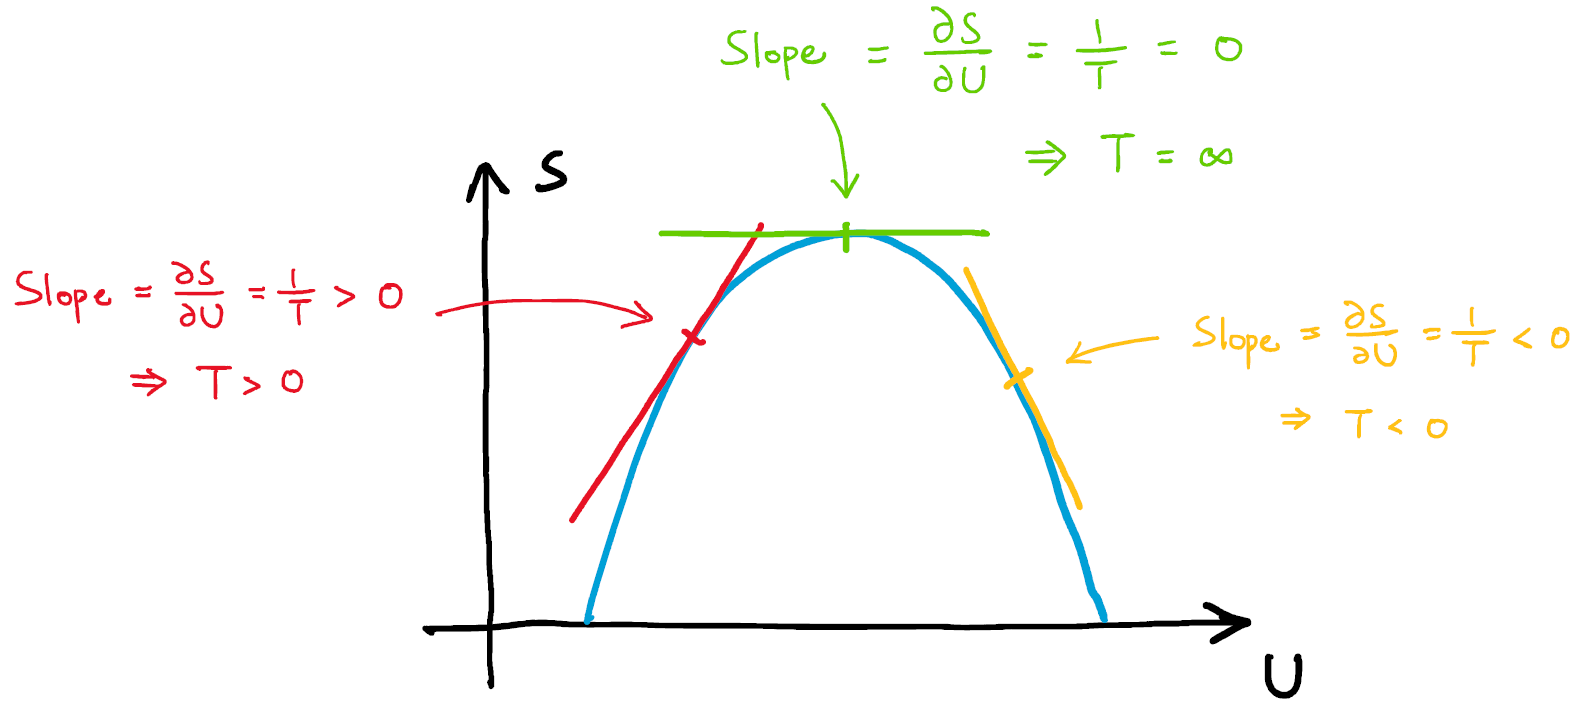
\includegraphics[width=\textwidth]{WU3}
    \end{minipage}
\end{center}

So the temperature scale defined by entropy is kind of "weird"...

\begin{center}
    \begin{minipage}{0.7\linewidth}
        \centering
        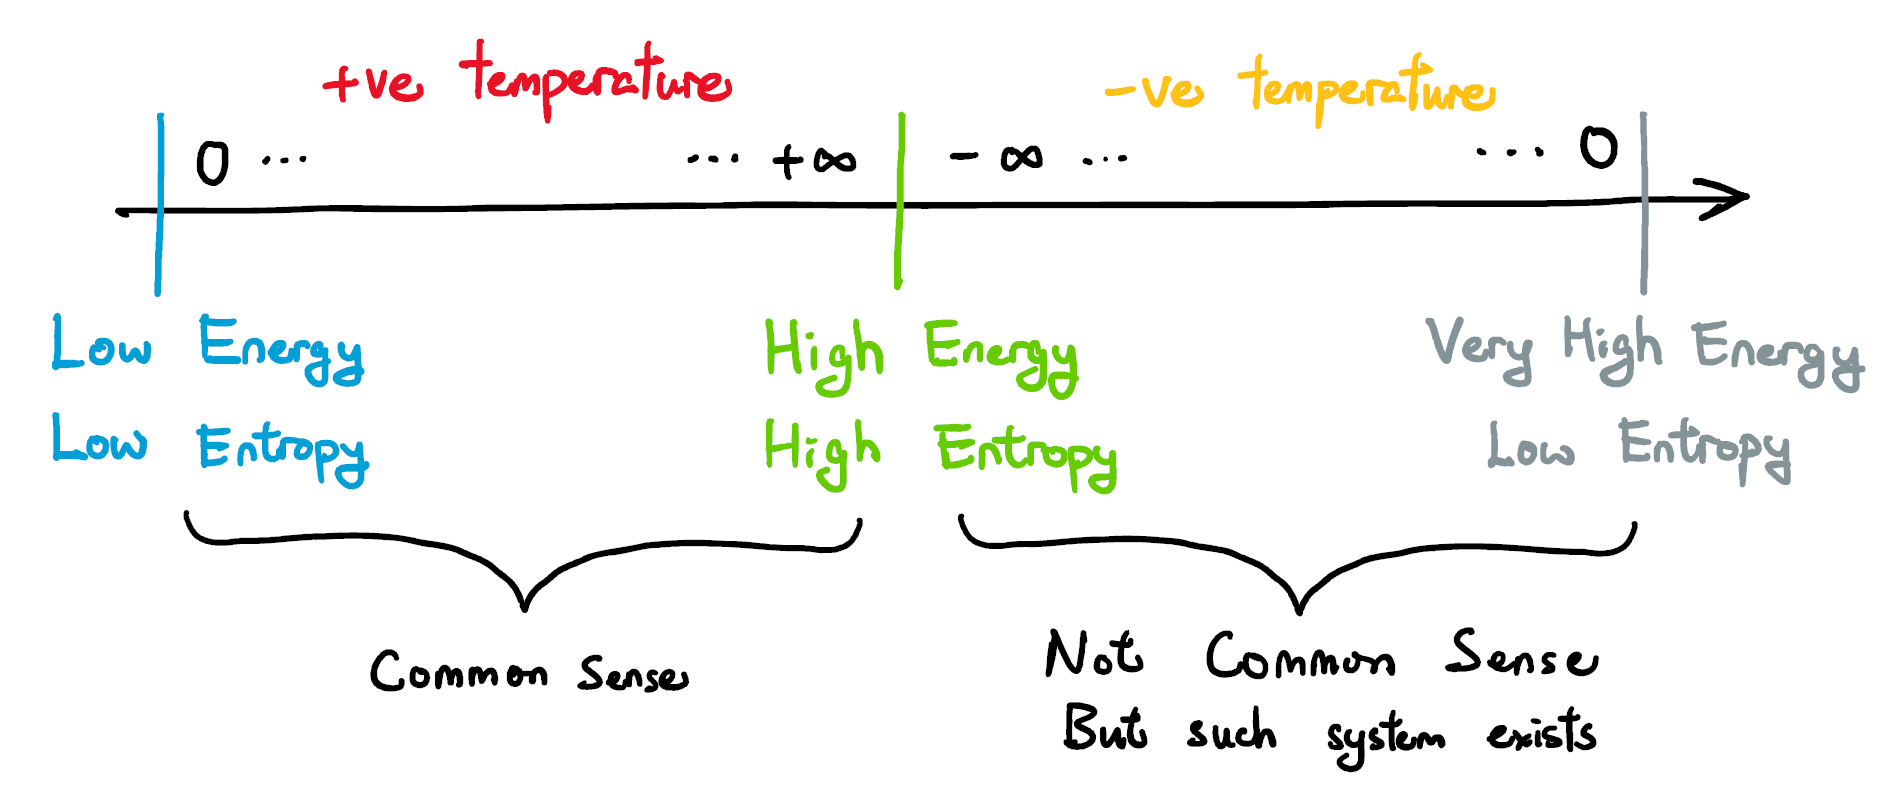
\includegraphics[width=\textwidth]{temp_scale}
    \end{minipage}
\end{center}

Under this definition,
\red{temperature is no longer about hot or cold.}\\

(And we still cannot go below $0$K!)


%%%
\theend
\end{document}